\chapter{Reference Data}

One proband has mounted two sensors on his bed right next to each other. Therefore each time series of the same day produced by these sensors should be really similar to each other. However a certain amount of noise will be expected. 

Anyway, in terms of similarity measurement, all time series pairs produced by these sensors will be as similar as one can get.

One of those pairs is defined as the reference time series pair. It is used as reference data for this project. It will set the ground truth for all the following distance and similarity measurements.

The following data sets were used to create the reference data:

\begin{itemize}
  \item sleepo\_2020-10-11\_to\_2020-10-12\_xxxxx.csv
  \item sleepo\_2020-10-11\_to\_2020-10-12\_yyyyy.csv
\end{itemize}



\section{Reference Data Granularity}
The reference time series are available in different granularities

\begin{itemize}
  \item 1 hour
  \item 30 minutes
  \item 5 minutes
  \item 1 minute
\end{itemize}

In order to create those granularities the raw time series had to be downsampled.
Missing observations were replaced using the custom forward fill algorithm. Then the data was resampled to the given granularity using a rolling mean approach.

The cleaning and creating of the reference data was done in the Jupyter Notebook "CleanReferenceData.ipynb".


\section{One Hour Granularity}

Figure \ref{fig:ref_ts_one_h_granularity} visualises the downsampled granularity of the one hour reference time series.
Table \ref{tab:ref_ts_one_h_granularity} gives an example on how the corresponding csv file looks like. The following data sets with other granularities will have the same format but are not displayed as table due to the larger number of rows.

\begin{figure}[h!]
	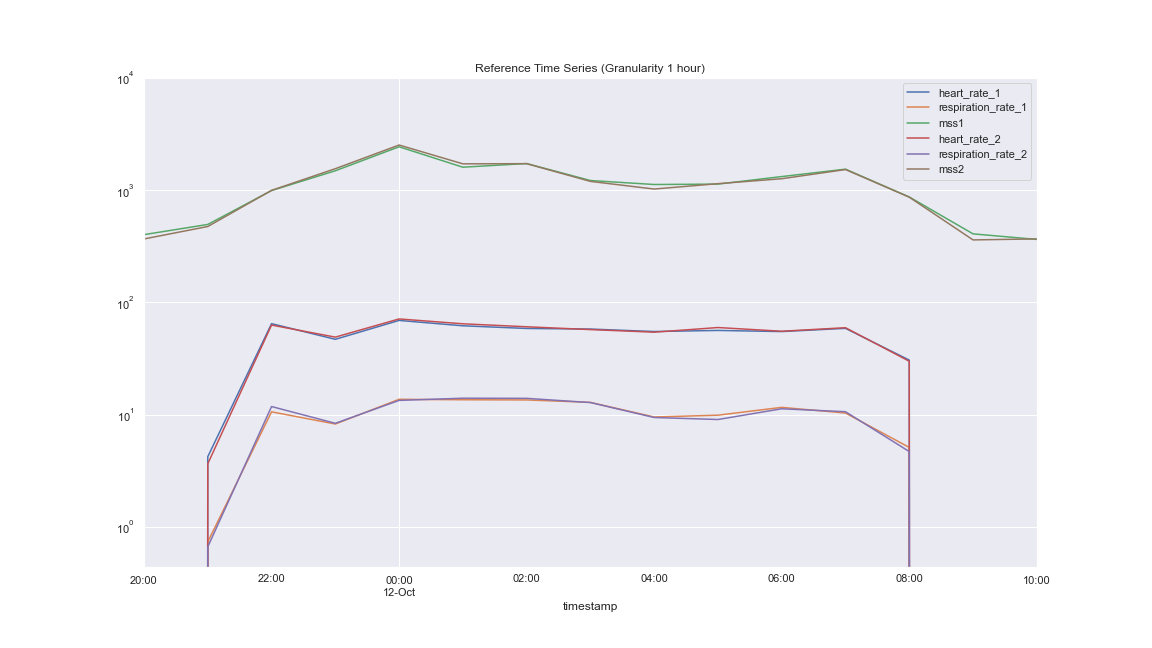
\includegraphics[width=1.1\textwidth]{/ref_timeseries_1hour.png}
	\caption{Reference data: One hour granularity visualisation}
	\label{fig:ref_ts_one_h_granularity}
\end{figure}


\begin{table}[h!]
\centering
\resizebox{\textwidth}{!}{
	\begin{tabular}{|c|c|c|c|c|}\hline%
		% specify table head
		\bfseries timestamp & 
		\bfseries heart\_rate\_1 &
		\bfseries respiration\_rate\_1 &
		\bfseries heart\_rate\_2 &
		\bfseries respiration\_rate\_2
		
		\csvreader[]{\myCleanedCsvDataPath/reference/ref_1hour.csv}{
			1=\myTS,2=\myHRa,3=\myRRa,
			4=\myHRb,5=\myRRb} % specify your columns here
			{\\\hline\myTS & \myHRa & \myRRa & 
			\myHRb & \myRRb}
		\\\hline	
	\end{tabular}
}
\caption{Reference data: One hour granularity data}
\label{tab:ref_ts_one_h_granularity}
\end{table}

This data is stored in \path{src/data/cleaned/reference/ref_1hour.csv}


\clearpage
\section{30 Minutes Granularity}

Figure \ref{fig:ref_ts_30_m_granularity} visualises the downsampled granularity of the 30 minutes reference time series.

\begin{figure}[h!]
	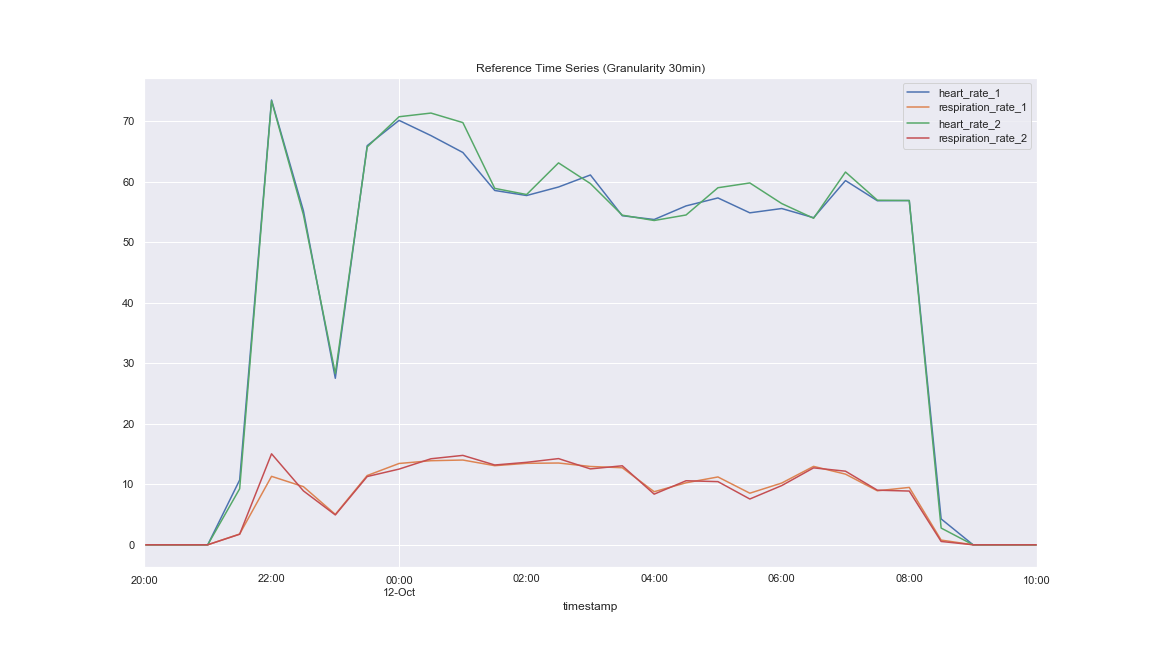
\includegraphics[width=1.1\textwidth]{/ref_timeseries_30min.png}
	\caption{Reference data: 30 minutes granularity visualisation}
	\label{fig:ref_ts_30_m_granularity}
\end{figure}

This data is stored in \path{src/data/cleaned/reference/ref_30min.csv}



\clearpage
\section{Five Minutes Granularity}

Figure \ref{fig:ref_ts_5_m_granularity} visualises the downsampled granularity of the five minutes reference time series.

\begin{figure}[h!]
	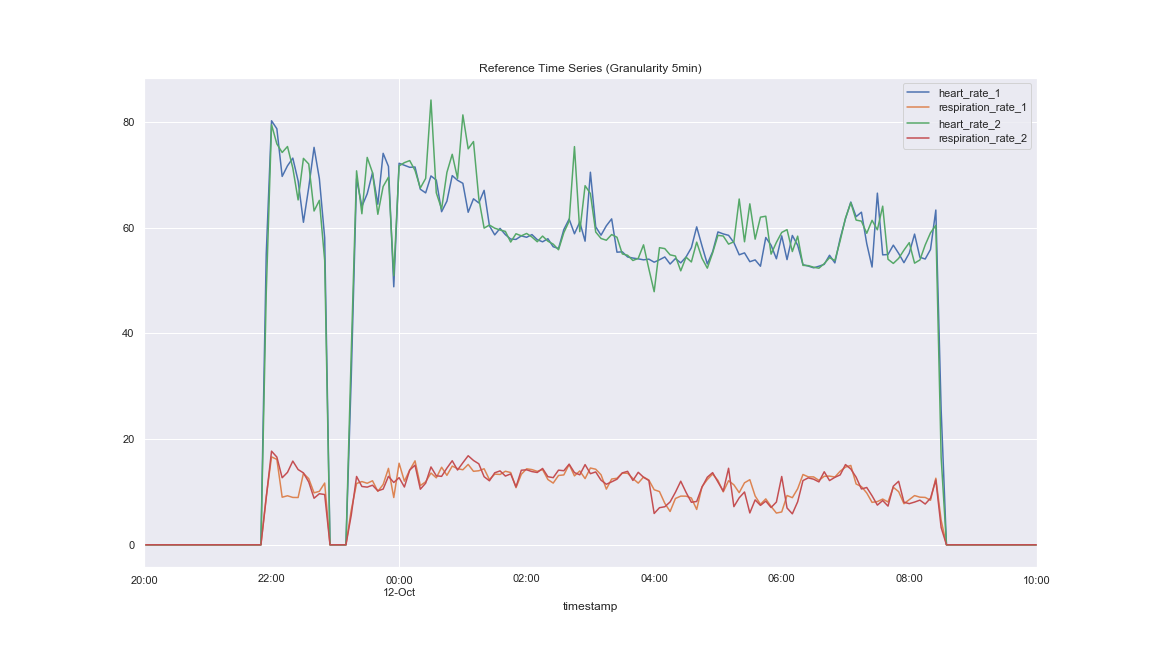
\includegraphics[width=1.1\textwidth]{/ref_timeseries_5min.png}
	\caption{Reference data: Five minutes granularity visualisation}
	\label{fig:ref_ts_5_m_granularity}
\end{figure}

This data is stored in \path{src/data/cleaned/reference/ref_5min.csv}



\clearpage
\section{One Minutes Granularity}

Figure \ref{fig:ref_ts_1_m_granularity} visualises the downsampled granularity of the one minute reference time series.

\begin{figure}[h!]
	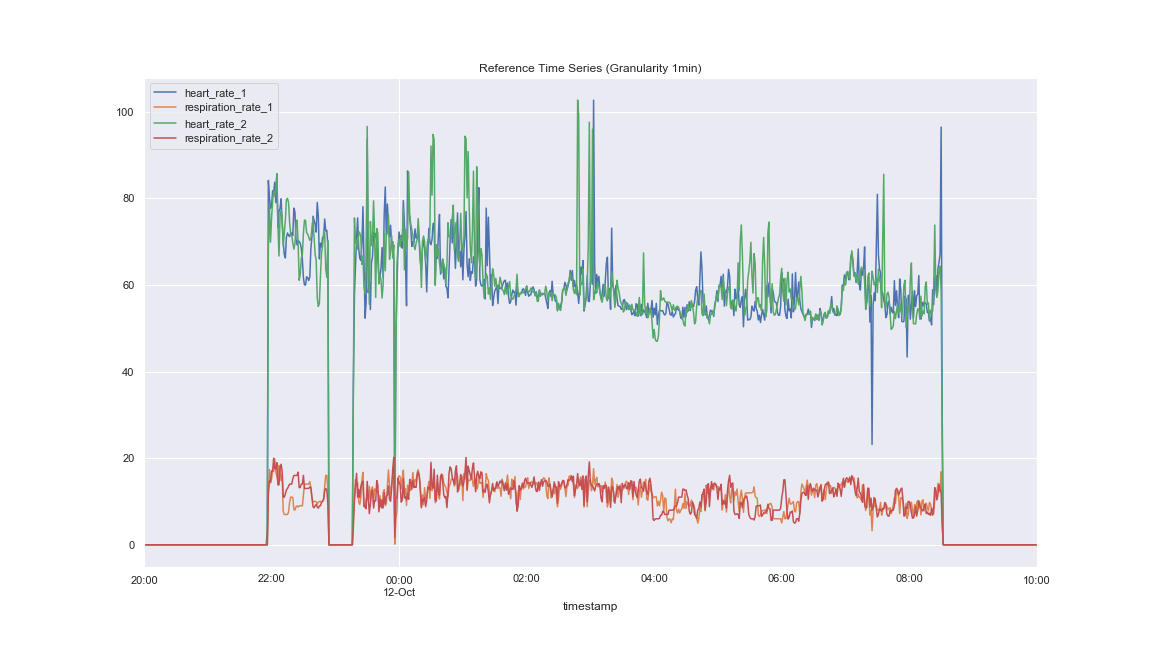
\includegraphics[width=1.1\textwidth]{/ref_timeseries_1min.png}
	\caption{Reference data: One minute granularity visualisation}
	\label{fig:ref_ts_1_m_granularity}
\end{figure}

This data is stored in \path{src/data/cleaned/reference/ref_1min.csv}



